\documentclass[draftcls, journal]{IEEEtran}
\usepackage{cite}
\usepackage[pdftex]{graphicx}
\usepackage[cmex10]{amsmath}
\interdisplaylinepenalty=2500
\usepackage{array}
\usepackage{dblfloatfix}

%%%Undefined packages
\usepackage{todonotes}
\usepackage{changes}
\definechangesauthor[name={Min Tan} color=orange]{MT}

\begin{document}
\title{A Single-Control-Circuit Multiple-Output Digital Low Dropout Regulator With Delay Switching}
\author{
        Kaixuan~Ye,~\IEEEmembership{Student Member,~IEEE,}
        Min~Tan,~\IEEEmembership{Member,~IEEE,}% <-this % stops a space
\thanks{The authors are with the School of Optical and Electronic Information,
Huazhong University of Science and Technology, Wuhan 430074, China (email:
mtan@hust.edu.cn).}
        }

\markboth{Journal of \LaTeX\ Class Files,~Vol.~14, No.~8, August~2015}%
{K.~Ye\MakeLowercase{\textit{et al.}}: DLDO Paper Draft}


\maketitle

\begin{abstract}
This paper presents a novel single-control-circuit multiple-output digital low dropout regulator (DLDO). Operating in the time division multiplexing mode, this DLDO can share a single control circuit and regulate multiple outputs at different time period. With the proposed delay switching technique, the cross regulation between different outputs can be totally eliminated. A prototype with two outputs was fabricated with UMC 130nm process and this approach can be extended to more outputs theoretically. As the DLDO design becomes more and more complicate and the control circuit takes up more and more area, this design points out a very promising way to save the total chip area.\\

\begin{IEEEkeywords}
Delay switching, time-division multiplexing, digital low dropout regulator.
\end{IEEEkeywords}
\end{abstract}

\section{Introduction}
To get a highly-efficient, highly-accurate supply voltage, hierarchical power managing networks are often employed in today's System-on-Chip(SoC) design \cite{original,AALDO,AALDO1,coarse-fine,pipeline,asynchrounous,recursive}. Fig \ref{hierarchical} depicts the general SoC hierarchical power managing network, firstly a highly-efficient buck converter scale down the battery voltage to the operating voltage of the SoC,then the output is connected to a low dropout regulator(LDO) to eliminate the ripple and finally the LDO provide a fine-grained supply voltage for the function units such as RFs, AD/DAC, I/Os.
 
\begin{figure}[h!]
    \centering
    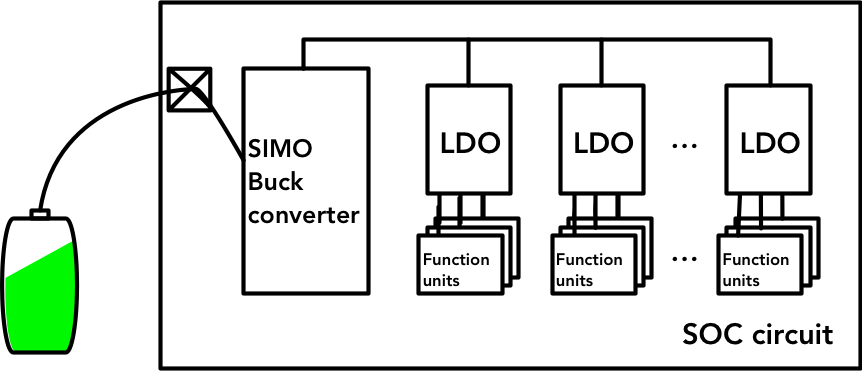
\includegraphics[width=\linewidth]{pic/DLDOsche/SOCcircuit.png}
    \caption{Hierarchical power managing network in SoC}
    \label{hierarchical}
\end{figure}
Traditionally, the LDOs are implemented with an error amplifier, power stage, feedback and other analog transient enhancement subcircuits to provide a highly-accurate supply\cite{ALDO1,ALDO2,ALDO3}. However, the analog LDO design become harder and harder with the SoC operating voltage scaling down, and the Digital LDO(DLDO) draw significant attention in recent years for its low voltage operation capability and process scalability. Fig\ref{basicDLDO} shows the original DLDO design proposed in\cite{original}. It consists of a clocked comparator, a bidirectional shift register, and a MOS array. When the output is below the reference, the shift register turn on a PMOS per clock, and vice versa. However, the original DLDO suffer from large drop voltage and ripple. Many advanced techniques proposed in \cite{AALDO, pipeline, coarse-fine, eventDriven,recursive} to handle these problems. In\cite{coarse-fine}, two MOS arrays with different size are employed. In steady state, the small MOS array is connected to the loop, and it switches to the large MOS array when the load changes. As a result, a relatively small drop voltage and ripple is realized simultaneously. In \cite{AALDO}, an additional analog assisted loop is added to further reduce the drop voltage. \cite{pipeline} apply a pipeline control but greatly increase the design complexity. In this paper, we adopt the design in \cite{AALDO} and \cite{coarse-fine} and realize a drop voltage around 100mV.

\begin{figure}[t]
    \centering
    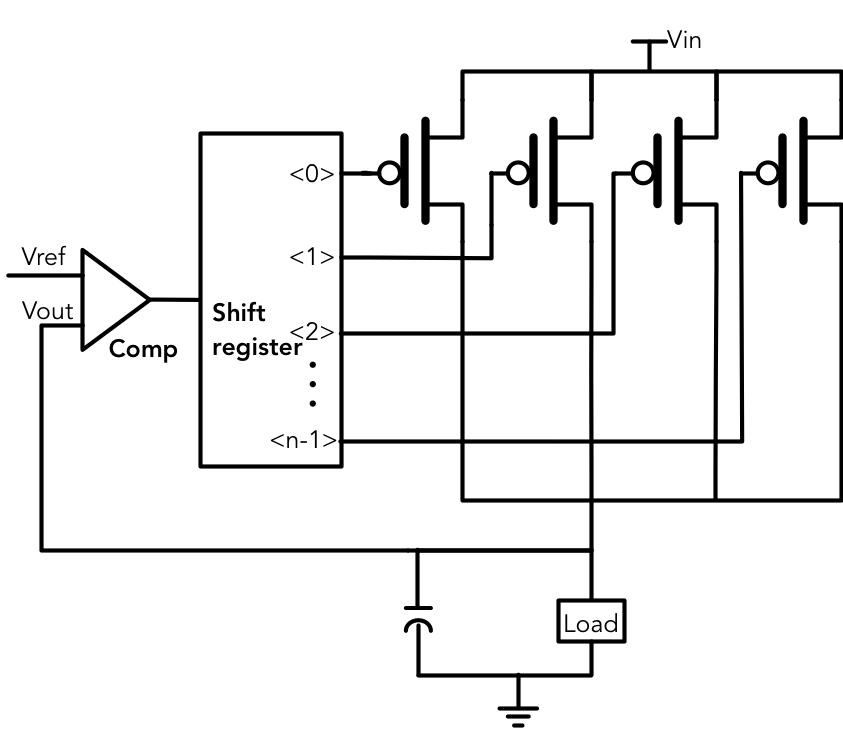
\includegraphics[width=\linewidth]{pic/DLDOsche/originalDLDO.png}
    \caption{The original DLDO design}
    \label{basicDLDO}
\end{figure}
As the function units in a typical SoC often have different requirements for the supply, multiple buck converters and LDOs are usually needed. And \cite{SIMODCDC,SIMODCDC1,SIMODCDC2} proposed a single input multiple output(SIMO) buck converter to save the chip area. The inductor in the SIMO buck converter is working time division multiplexed, i.e. the inductor is connected to different paths at different time periods, consequently it can serve many LDOs while only use one inductor, which greatly reduce the needed chip area.

In the following parts of this paper, we will first discuss the TDM scheme applied in many circuit designs in section II, then in section III, we will talk about the architecture and working principles of the proposed design. In section IV, the implementation and design considerations of the circuit will be discussed. And in section V, we present the experiment results of the proposed design, and finally we draw a conclusion in section VI.
%%This paragragh needs further tuning.
\section{TDM scheme}
In some circuit designs, a certain building block takes up a great percentage of the whole chip area. Instances are like the controller in the micro ring modulator, the inductor in the DC-DC converter, and the compensation capacitor in the low dropout regulator (LDO). Normally, more than one such circuits are needed in a SoC circuit, and the most straightforward way to realize it is to implement N single output such circuits. However, one the one hand, this immoderately consumes the chip area, and on the other hand, passive devices like inductor and capacitor may bring about great noise to the circuit. To solve this problem, the TDM scheme has been applied to many circuits and have achieved great success.
\subsection{TDM micro ring modulator}
In the burgeoning integrated optoelectronics design, the silicon Micro Ring Modulator (MRM) is believed to be the most important device to realize optical interconnect, which have been proposed to displace electrical interconnects as the next generation I/O links due to its ultra-wide bandwidth and low loss advantages \cite{wangzhicheng}. However, as is highly sensitive to the thermal fluctuation, the MRM usually requires a feedback control circuit to stabilize its resonant wavelength. Normally, the control circuit is much larger than the micro ring, and in order to save chip area, \cite{wangzhicheng} have proposed a TDM scheme to simultaneous lock the wavelength of multiple silicon micro rings.
\begin{figure}[t!]
    \centering
    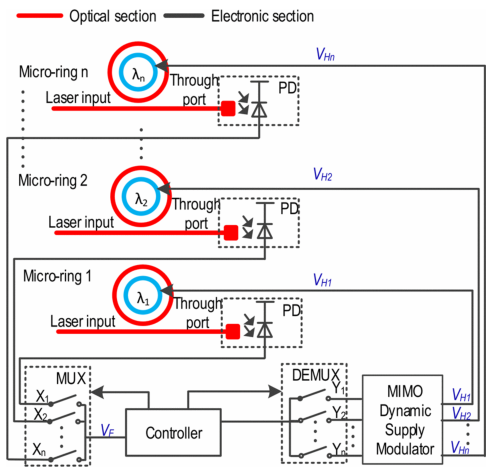
\includegraphics[width=\linewidth]{pic/TDM/MRM.pdf}
    \caption{The TDM scheme applying in micro ring design}
    \label{fig:MRM}
\end{figure}

Fig.\ref{fig:MRM} shows the working principle of the TDM scheme. The MUX and DEMUX connect the photodetector(PD) and its corresponding supply modulator to the controller at different time intervals, as a result, the shared controller, which is composed of an ADC, a MCU and a DAC, can cope with the imformation of different micro rings at different time period.

\subsection{SIMO DC-DC Converter}
\begin{figure}[t!]
    \centering
    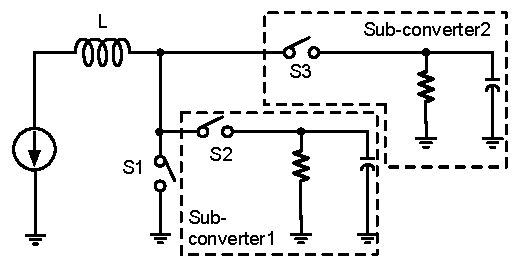
\includegraphics[width=\linewidth]{pic/TDM/DCDC.pdf}
    \caption{The TDM scheme applying in DC-DC converter}
    \label{fig:DCDC}
\end{figure}
\begin{figure}[t!]
    \centering
    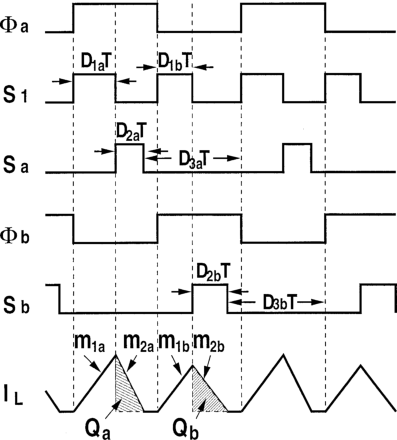
\includegraphics[width=0.8\linewidth]{pic/TDM/DCDC-timing.pdf}
    \caption{Timing diagram of the SIMO DC-DC converter}
    \label{fig:DCDC-timing}
\end{figure}
The DC-DC converters are usually applied in the SoC power management circuit for its high converting efficiency. However an off-chip inductor is required for every DC-DC converter. When multiple power domains exists, which is quite normal in a SoC circuit, multiple DC-DC converters are implemented conventionally. This not only increase the number of required on-chip pads, but also may bring about great noise to the circuit. In \cite{SIMODCDC} an single inductor multiple output (SIMO) DC-DC buck converter is proposed, as is shown in Fig\ref{fig:DCDC}.

Both subconverter a and converter b are operating in DCM mode, and Fig\ref{fig:DCDC-timing} explicitly interprets the working principle. $\Phi a$ and $\Phi b$ are two complementary phase signals which indicate the regulating period. When $\Phi a = 1$, the subconverter A is connected to the inductor, and the current through the inductor ramps up at $D_{1a}T$ and ramp down at $D_{2a}T$. Similar current behavior happens again when $\Phi b =1$, and the current is assigned to different subconverters without affecting each other. 

\subsection{the proposed TDM DLDO}
\begin{figure}[t!]
    \centering
    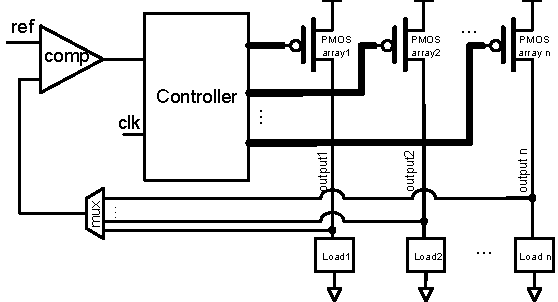
\includegraphics[width=\linewidth]{pic/TDM/TDMDLDO.pdf}
    \caption{the proposed TDM DLDO}
    \label{fig:TDMDLDO}
\end{figure}
Contrary to the analog counterpart, in the Digital LDO design, the control circuit takes up a great percentage of the whole chip area, even greater than the power stage. The control circuit is usually composed of shift registers, and each power MOS array unit needs a shift register stage. So it would be very promising if we can share the control circuit between different outputs like the TDM MRMs and the SIMO DC-DC converters.

Fig.\ref{fig:TDMDLDO} shows our proposed TDM DLDO, and the working principle is very simple and similar to the TDM MRM. The mux select different outputs to the comparator at certain time periods. Then the comparator compares the output voltages with the reference, and the comparison result serves as the input signal of the controller, which finally determines the states of the power PMOS array. Multiple outputs share the single control circuit at different time period, so the proposed DLDO is operating at TDM mode.

\section{Architecture and working principle of the proposed design}
\subsection{Architecture}
The architecture of the proposed TDM DLDO is shown in Fig.\ref{fig:TDMDLDO}. It mainly composes of a comparator, a output MUX, an analog-assisted loop, two groups of latches, namely lat\_0 and lat\_1 in the diagram, two groups of PMOS arrays, in each group the size of the "coarse" PMOS array unit is 9 times larger than that of the "fine" PMOS array unit, and two groups of shift register, which are coarse and fine shift registers. The shift registers determine the states of the PMOS arrays and can be asynchronously set/reset by the special set/reset block.  

In the whole diagram, not only the comparator, but also the analog-assisted loop and the coarse and fine shift registers are shared the by two outputs. The latches serve as the buffer stage, which also exist in many other DLDO designs\cite{AALDO,AALDO1}. Apart from that, only an additional multiplexer, the "outputMux" is added to the circuit, which scarcely bring any additional area to the whole chip. In other word, we almost double the efficiency of the control circuit in terms of area.
\subsection{Delay switching technique}
\begin{figure}[t!]
    \centering
    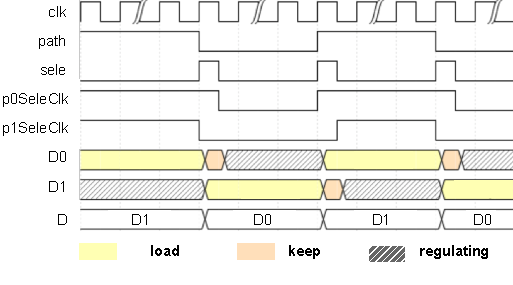
\includegraphics[width=\linewidth]{pic/struc/timing.pdf}
    \caption{Timing diagram of the proposed design}
    \label{fig:timing}
\end{figure}
\begin{figure}[t!]
    \centering
    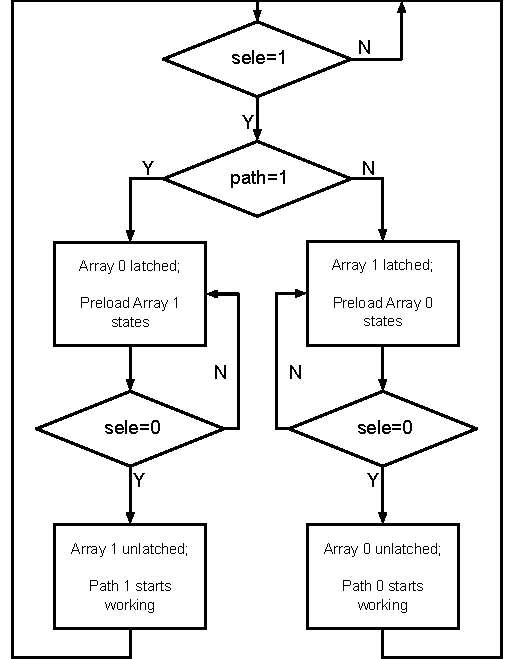
\includegraphics[width=0.9\linewidth]{pic/struc/flowChart.pdf}
    \caption{Flowchart of the delay switching process}
    \label{fig:flowchart}
\end{figure}
\begin{figure*}[t!]
    \centering
    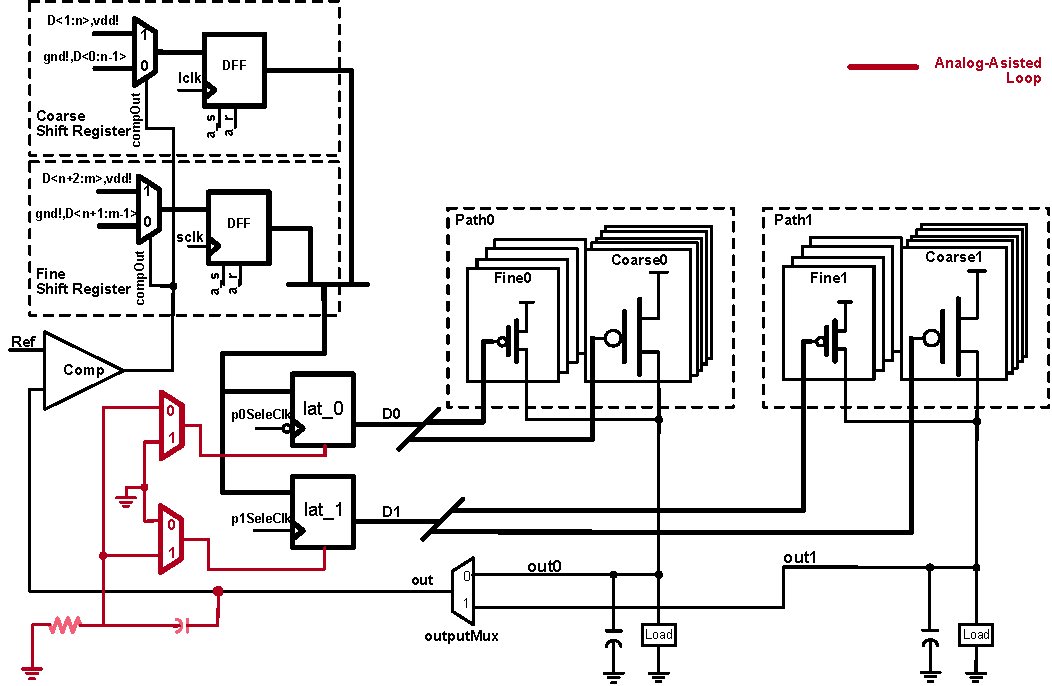
\includegraphics{pic/struc/sche.pdf}
    \caption{Structure of the proposed TDM DLDO}
    \label{fig:diag}
\end{figure*}
\begin{figure}[t!]
    \centering
    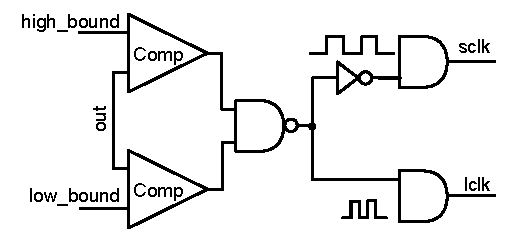
\includegraphics[width=0.7\linewidth]{pic/struc/peak.pdf}
    \caption{Peak detector}
    \label{fig:peak}
\end{figure}
In the TDM scheme design, cross coupling is one of the most salient problems. In the SIMO DC-DC converter proposed in \cite{SIMODCDC}, the subconverters work in DCM mode, so there is a inherit guard period  between different regulating periods when the current running through the inductor stays zero. And in the TDM micro ring proposed in\cite{wangzhicheng}, a guard period is also inserted between different processing periods to avoid the cross coupling between different outputs. In DLDO, the PMOS arrays are controlled by the shift registers. If we share the shift registers without protection, the states of other PMOS array may be loaded during the switching period and great cross-channel coupling occurs. To solve this problem, we propose the delay switching technique.

Fig.\ref{fig:timing} shows the timing diagram of our design, "clk" is the system clock and "path" is the path switching signal. The "sele" signal generates a pulse at every rising and falling edges of the "path". And "P0/1SeleClk" are the derivative signal from "path" and "sele", which drives the latch groups. “D0/1” stands for the states of the PMOS array, and “D” stands for the outputs of the shift register. 

The working principle of the delay switching technique is best interpreted with the reference of the flowchart shown in Fig.\ref{fig:flowchart}. At every switching instance, the "sele" signal generates a pulse, in other word, "sele" = 1 during this period. If "path" = 1 at that time, meaning that the control circuit is to be connected to the power PMOS array 1, then the power PMOS array 0 is latched by "lat\_0", so the output voltage at path 0 maintains if the load does not change. Meanwhile, the asynchronous set/reset block load the previously latched states of the array 1 to the shift registers. After all the data are loaded and the pulse at "sele" signal disappears, then the power PMOS array 1 is officially connected to the shift registers. And the shift registers starts to control the states of the power PMOS array according to the comparison results until the next switching instance happens. As we load its previous states before we connect one path to the control circuit, no cross-channel coupling should exist.

\subsection{The shared analog-assisted loop}
When the load switch from light to heavy, the power PMOS array may not able to provide enough current, and an undershoot occurs at the output. Normally, the shift register should turn on the array units to provide more current. However, as is shown in Fig.\ref{fig:aaloop}a, the array unit remains high until the clock arrives and the shift register transfer the comparison result to the array. As a result, the undershoot may be very large in the DLDO. To solve this problem, \cite{AALDO} proposed the analog-assisted loop. The working principle is clear, as is shown in Fig\ref{fig:aaloop}b, if we can feedback the undershoot to the gate of the array unit, the unit can be at the half-open state before the clock arrive, so the undershoot is greatly reduced. To realize it, an RC loop connect the output and the ground of the inverter buffer as is shown in \ref{fig:latch}. So whenever an undershoot occurs, the buffer can sense it and tranfer it to the array instantly.

However, the on-chip capacitors and resisters consume lots of area, so if we can share the analog-assisted loop, the area efficiency can be further increased.
\begin{figure}[t!]
    \centering
    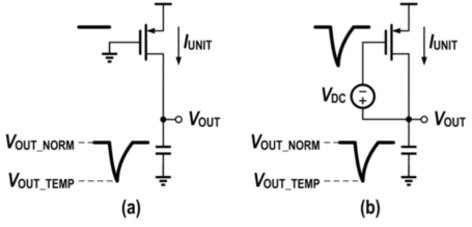
\includegraphics[width=\linewidth]{pic/struc/aaloop.pdf}
    \caption{Comparison between with AA loop and without AA loop}
    \label{fig:aaloop}
\end{figure}
\begin{figure}[t!]
    \centering
    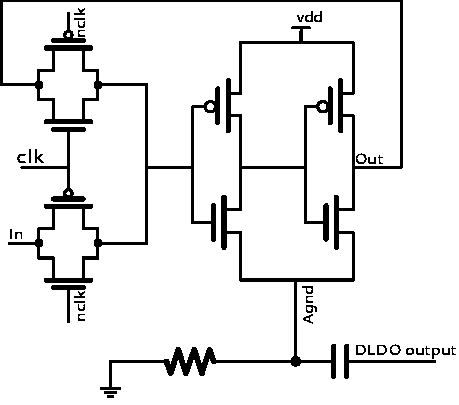
\includegraphics[width=0.9\linewidth]{pic/struc/latch.pdf}
    \caption{The latch structure appied in "lat\_0" and "lat\_1"}
    \label{fig:latch}
\end{figure}


\bibliographystyle{ieeetr}
\bibliography{05ref}
\end{document}


